\chapter{\MakeUppercase{Clasificación no supervisada de ruido combinacional por medio del tiempo de vuelo}}

En este apartado se analizaron los eventos detectados por MuTe mediante las mediciones del ToF y GMM. Los eventos se clasifican como correlacionados y no correlacionados por medio del tiempo de vuelo (ToF).  Las partícula correlacionadas e individuales su tiempo de vuelo oscila entre 2 a 30$ ns$, mientras que las partículas no correlacionadas, la diferencia temporal entre las 2 partículas es $> 300 ns$, revisar Fig. \ref{placas}. La probabilidad de que ocurra un evento por partículas no correlacionadas con un diferencia temporal $<  200ns$ es de $\med 0,05\%$ \footcite{jesusP}.

\begin{figure}[h!]
\begin{center}
\caption{Partículas incidentes que cruzan los paneles. Estos se clasifican en correlacionados (verde oscuro), no correlacionados (verde claro), y eventos simples (rojo).}
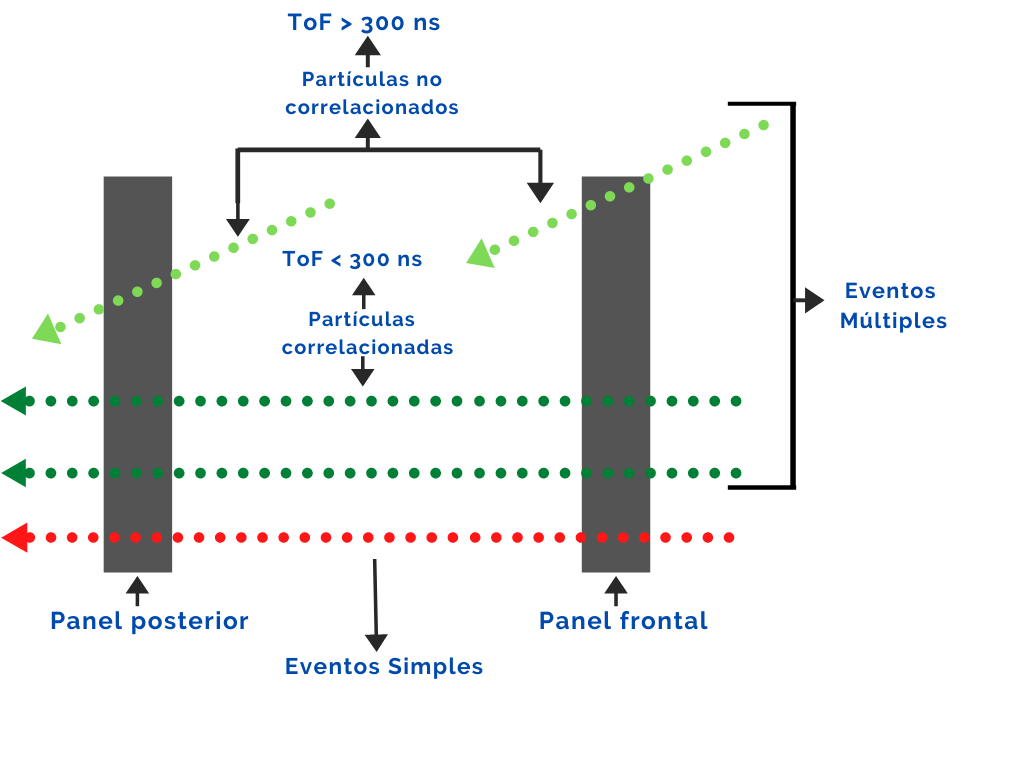
\includegraphics[width=0.71\textwidth]{Figures/imagenes/panel.png}
\label{placas}
\end{center}
\end{figure}

\section{Eventos de partícula simple, correlacionados y no-correlacionados teniendo en cuenta el ToF }


\subsection{Tratamiento y análisis de datos.\\}

Inicialmente, se hizo una visualización de los datos para analizar la relación que tienen los eventos con las etiquetas teniendo en cuenta la información a-priori. La primera gráfica muestra el tiempo de vuelo de cada uno de los eventos. En la Fig. \ref{300} se observa una aglomeración de datos correspondientes a los eventos correlacionados (ToF < 300ns). Los no correlacionados se dispersan uniformemente sobre los valores > 300ns.

El histograma de frecuencia, evidencia la distribución de los eventos con ToF $< 300 ns$, como se muestra en la Fig. \ref{ocho}.\\

\begin{figure}[h!]
\begin{center}
\caption{ Tiempo de vuelo de cada evento. Un umbral en 300ns (linea negra) permite dividir los eventos correlacionados (< 300ns) de los no-correlacionados (> 300ns).}
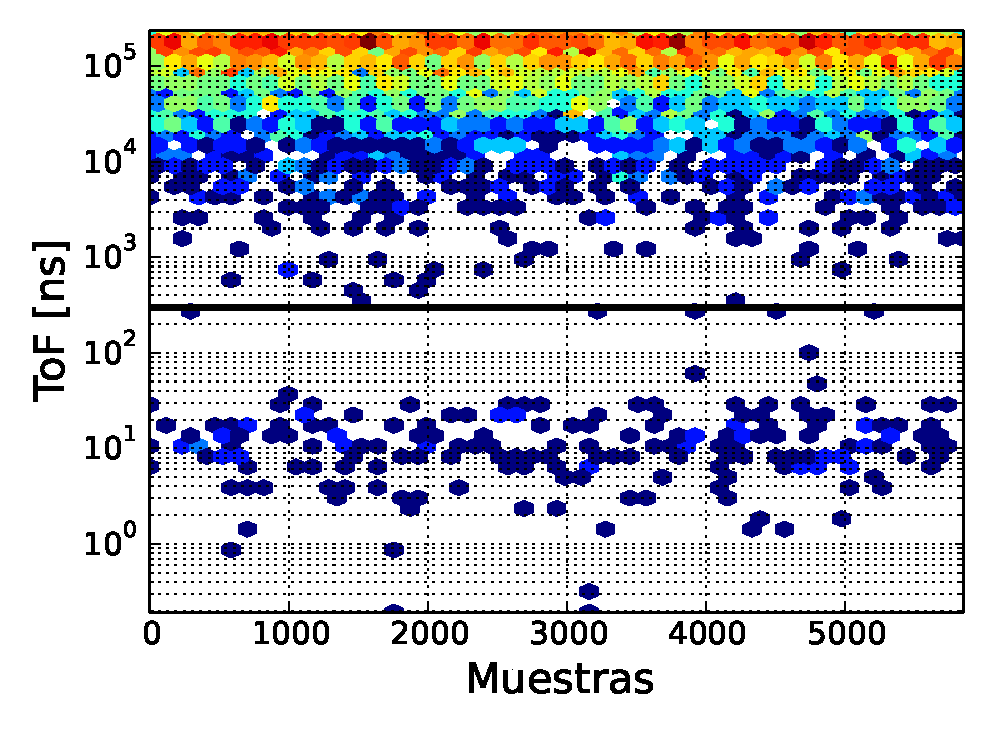
\includegraphics[width=0.7\textwidth]{Figures/imagenes/ag.eps}
\label{300}
\end{center}
\end{figure}


También se visualizaron los datos en orden logarítmico para corroborar la conclusión obtenida de las dos gráficas anteriores. En la Fig. \ref{nueve}, se evidencia una concentración de muestras alrededor de 10 ns corroborando un mayor número de eventos correlacionados. Ubicadas estas zonas de interés, se parametrizan los datos por medio de distribuciones.\\



\begin{figure}[h!]
\begin{center}
\caption{ Histograma de frecuencia de los datos del tiempo de vuelo.}
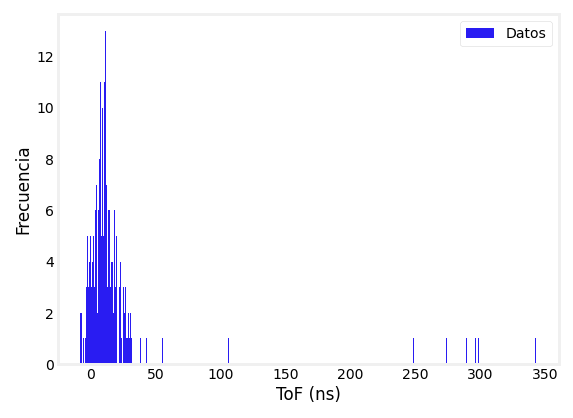
\includegraphics[width=0.7\textwidth]{Figures/imagenes/7.png}

\label{ocho}
\end{center}
\end{figure}

\begin{figure}[h!]
\begin{center}
\caption{Tiempo de vuelo en orden logarítmico. Se distinguen los eventos de partícula simple y correlacionadas con un ToF menor a 300ns, mientras que los eventos no correlacionados tienen ToF mayores a 300 ns  }
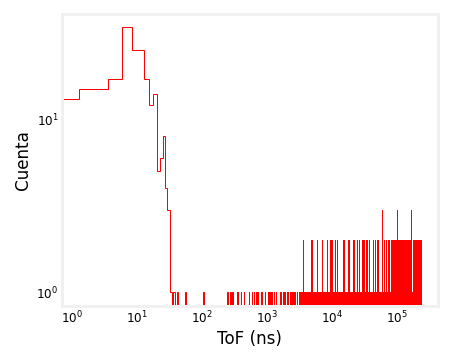
\includegraphics[width=0.6\textwidth]{Figures/imagenes/8.png}

\label{nueve}
\end{center}
\end{figure}


\section{Clasificación y segmentación.}
 Bajo las métricas del ToF se ingresaron los datos a GMM para parametrizar cada componente. Se trabajó con 5883 datos definiendo parámetros iniciales como: el número de componentes (2), el número de iteraciones (1000), los pesos de cada componente (0.9 para correlacionados y 0.1 para no-correlacionados) y el número de iniciaciones que tuvo el modelo (5). Todo escogido para que se ajustara mejor a los eventos de partícula simple y correlacionada.
 
 Al parametrizar las componentes, se validó el modelo con los datos reales. De los parámetros de salida se tomó la varianza (76.80), la media (10.22) y los pesos de las componentes (0.96 y 0.037) para empezar con la separación de los eventos correlacionados y la eliminación de los no-correlacionados. Como se ve en la Fig. \ref{diez}).\\
 \\
 \\


\begin{figure}[h!]
\begin{center}
\caption{ToF $< 300  ns$. Eventos correlacionados. Los datos entregados por el detector y el modelo ajustado, muestran que los eventos se concentran en un ToF menor a 40ns.}
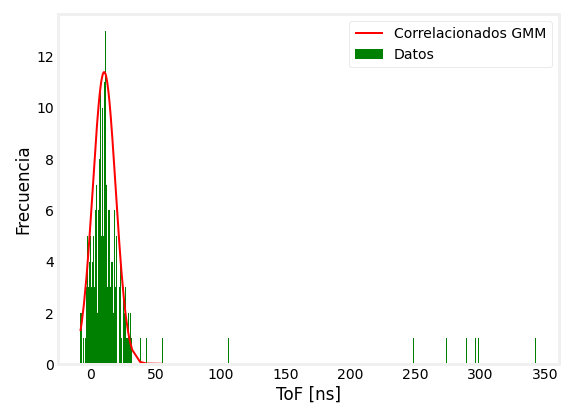
\includegraphics[width=0.75\textwidth]{Figures/imagenes/9.png}

\label{diez}
\end{center}
\end{figure}

\chapter{CLASIFICACIÓN NO SUPERVISADA DE LOS MUONES DE BAJO MOMENTUM.}
Para la discriminación de los muones de bajo momentum (<1 GeV/c), se trabajó con la relación de dos variables: el momento y el ToF. Se graficó en escala logarítmica para ver la relación entre las 2 variables e identificar su umbral.  Los muones con momento menor a $1 GeV/c$ son filtrados ya que sufren una dispersión angular que afecta la resolución espacial del MuTe. El proceso de clasificación se llevó a cabo gracias a algoritmos de clasificación no supervisada.


\section{Manejo de variables}

Inicialmente se eliminaron datos NaN de los datos crudos que dificultaban el procesamiento. Los datos resultantes se redujeron $\sim$ en un 40$\%$. En esta parte del proyecto ya se filtró la mayoría de las fuentes de ruido. 
Tras relacionar el ToF y el momentum, ver Fig.(\ref{doce}), se clasificó los muones de interés que presentan un momentum mayor a 1GeV/c. A continuación se explica la relación entre el ToF y el momento.\\ 

\begin{figure}[h!]
\begin{center}
\caption{ToF vs momentum. El 54$ \%$ de las partículas tiene momentum mayor a 1GeV/c (linea púrpura).}
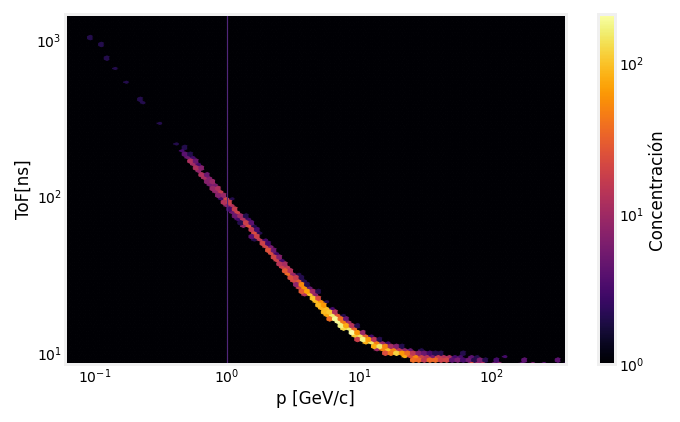
\includegraphics[width=0.75\textwidth]{Figures/imagenes/11.png}

\label{doce}
\end{center}
\end{figure}

\section{Estimación de momentum}
El sistema de ToF de MuTe mide el tiempo de vuelo que tardan las partículas cargadas de energía en atravesar un determinada trayectoria en el hodoscopio. Utilizando el ToF y la energía depositada en el WCD, MuTe estima el momentum de todas las partículas que ingresan al detector, estableciendo umbral para discriminar las partículas de baja energía (< 1Gev/c) \footcite{jesusP}.

La estimación del momentum se lleva a cabo con el fin de encontrar los eventos que sufren de dispersión múltiple. El cálculo del momentum depende de 2 variables, el ToF y la distancia recorrida entre las placas, que se define en la Ecuación ( \ref{MOM}).

\section{Clasificación}

En el proceso de clasificación se probaron varios métodos: \textit{Aglomerative Clustering}  \textit{Kmeans}, \textit{PCA} y \textit{ Spectral Clustering} . Con \textit{Aglomerative Clustering} y \textit{Kmeans} hubo un mejor ajuste de los datos, como se ve en la Fig. (\ref{ACvskM}). 
Luego estos clasificadores se probaron con diferente número de clúster, para compararlos minuciosamente mediante la medición de la precisión. \\




\section{\textbf{Análisis de Resultados.}}

\begin{figure}[h!]
\begin{center}
\caption{ToF vs momento entregados por los clasificadores \textit{AgglomerativeClustering} y \textit{Kmeans}, se muestra la comparativa de 2 a 4 clusters, con el umblar en 1GeV/c. (linea roja)}
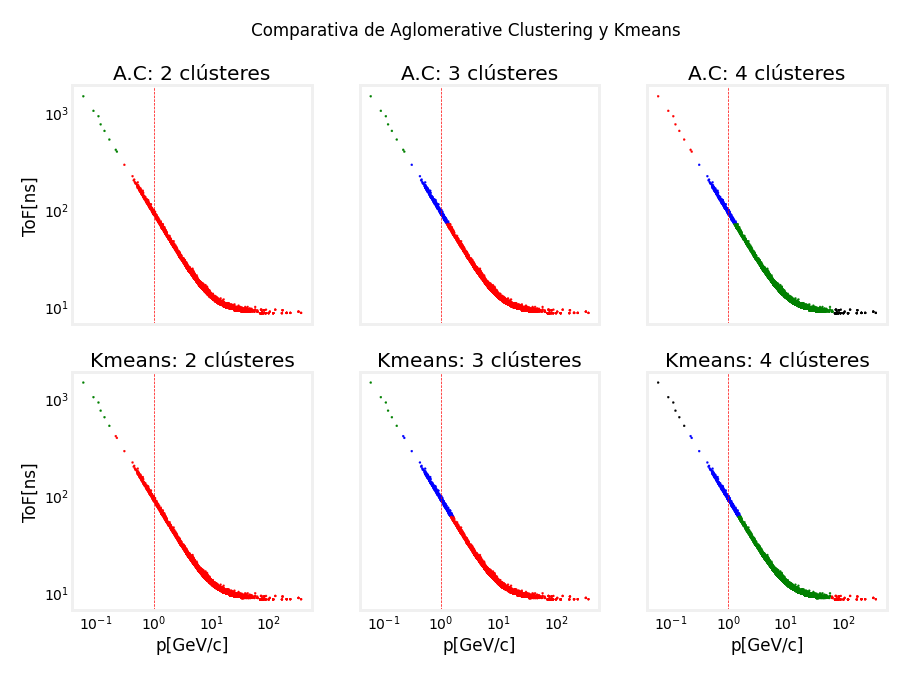
\includegraphics[width=0.9\textwidth]{Figures/imagenes/AK.png}
\label{ACvskM}
\end{center}
\end{figure}

Para la decisión final se tuvo en cuenta 2 factores: la precisión de la clasificación y la complejidad computacional.  En este orden de ideas, según los resultados obtenidos se escogieron tres clústeres con el algoritmo de \textit{Aglomerative Clustering}. Al aumentar el volumen de datos y el número de clústeres, se afecta el funcionamiento fluido del algoritmo, así que se validó con el resultado más óptimo.\\


\begin{figure}[h!]
\begin{center}
\caption{ToF vs momento entregados por los clasificadores \textit{Aglomerative Clustering} y \textit{Kmeans}, se muestra la comparativa de 2 a 4 clusters. Muestra el porcentaje de cada grupo en cada cluster.}
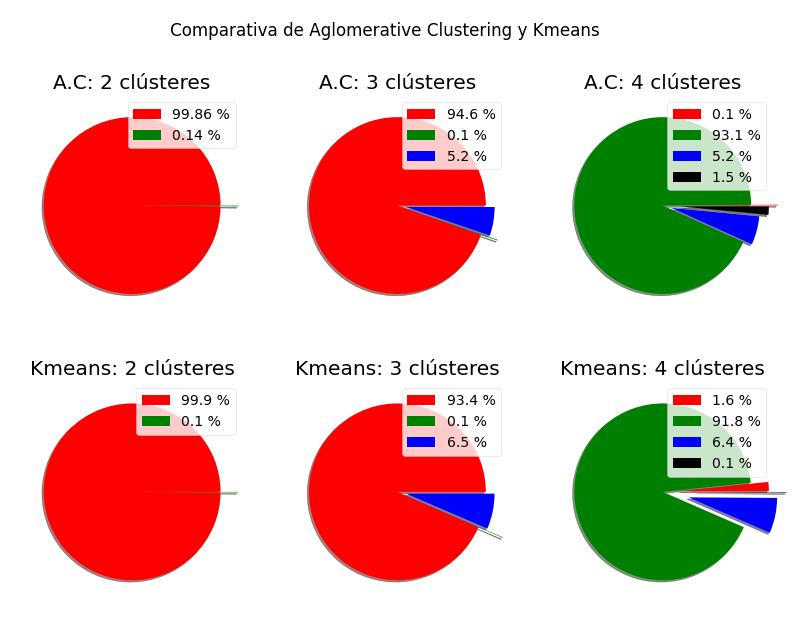
\includegraphics[width=0.9\textwidth]{Figures/imagenes/tor.png}
\label{ACvskM1}
\end{center}
\end{figure}

En términos generales $\sim$ el 90 $\%$ de los eventos estaban en la zona de aceptación (>1 GeV/c), esta condición se presento en todos los clusteres. Otra cosa que cabe mencionar, es que en todos los clusters el grupo de mayor cantidad de eventos estuvo estrictamente después del umbral de 1GeV/c como se muestra en la Fig. \ref{ACvskM}. 


% \begin{figure}[h!]
% \begin{center}
% \caption{\textit{Aglomerative Clustering} y \textit{Kmeans}, se muestra la comparativa de 2 a 4 clusters. Relaciona cada grupo con su respectivo número de muestras.}
% 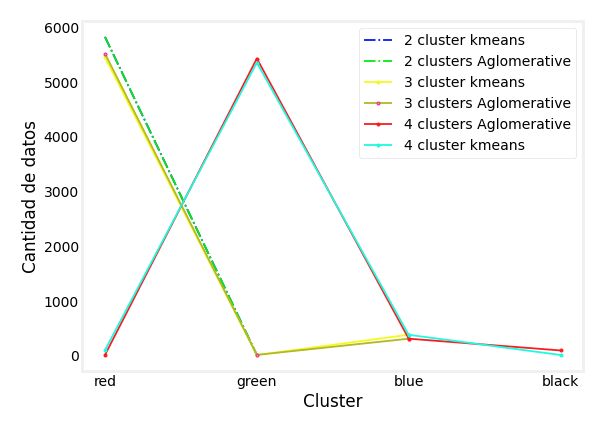
\includegraphics[width=0.65\textwidth]{Figures/imagenes/coin.png}
% \label{ACvskM2}
% \end{center}
% \end{figure}

No hubo diferencias significativas en los resultados entre los 2 algoritmos al evaluarse con el mismo número de clusters, diferían por  $\sim$3\% (200 datos). La diferencia a validar fue la posición del grupo en la muestra de datos. Por ejemplo en 2 clusters con \textit{Kmeans}, el grupo \textit{rojo} con 5817 datos, fue el menos preciso con respecto al umbral de 1GeV/c. Para 3 clusters se tuvo una mejor precisión, con un 94.6\% para \textit{AgglomerativeClustering} y 93.4\% para \textit{Kmeans} como se puede ver en la Fig. \ref{ACvskM1}.

